%%%%%%%%%%%%%%%%%%%%%%%%%%%%%%%%%%%%%%%%%  
% FRI Data Science_report LaTeX Template  
% Version 1.0 (28/1/2020)  
%   
% Jure Demšar (jure.demsar@fri.uni-lj.si)  
%  
% Based on MicromouseSymp article template by:  
% Mathias Legrand (legrand.mathias@gmail.com)   
% With extensive modifications by:  
% Antonio Valente (antonio.luis.valente@gmail.com)  
%  
% License:  
% CC BY-NC-SA 3.0 (http://creativecommons.org/licenses/by-nc-sa/3.0/)  
%  
%%%%%%%%%%%%%%%%%%%%%%%%%%%%%%%%%%%%%%%%%  
  
  
%----------------------------------------------------------------------------------------  
%	PACKAGES AND OTHER DOCUMENT CONFIGURATIONS  
%----------------------------------------------------------------------------------------  
\documentclass[fleqn,moreauthors,10pt]{ds_report}  
\usepackage[english]{babel}  
  
\graphicspath{{fig/}}  
  
  
  
  
%----------------------------------------------------------------------------------------  
%	ARTICLE INFORMATION  
%----------------------------------------------------------------------------------------  
  
% Header  
\JournalInfo{FRI Natural language processing course 2025}  
  
% Interim or final report  
\Archive{Project report}   
%\Archive{Final report}   
  
% Article title  
\PaperTitle{Conversational Agent with Retrieval-Augmented Generation}   
  
% Authors (student competitors) and their info  
\Authors{Luka Dragar, Urša Keše, Ožbej Pavc}  
  
% Advisors  
\affiliation{\textit{Advisors: Aleš Žagar}}  
  
% Keywords  
\Keywords{Retrieval-Augmented Generation, Conversational AI, Real-time Information Retrieval, Web Scraping, Natural Language Processing, Knowledge-Augmented Chatbots}  
  
\newcommand{\keywordname}{Keywords}  
  
  
%----------------------------------------------------------------------------------------  
%	ABSTRACT  
%----------------------------------------------------------------------------------------  
  
\Abstract{  
This project implements an advanced conversational agent that leverages Retrieval-Augmented Generation (RAG) to enhance response quality and factual accuracy. Unlike traditional chatbots relying solely on pre-trained knowledge, our system incorporates real-time web scraping capabilities to retrieve up-to-date information from the internet. Our implementation features a modular pipeline architecture that includes query enhancement, web search via SearXNG, content extraction, semantic chunking, embedding-based retrieval with reranking, and optimized context building for LLM integration. All components are self-hosted and open source, making it flexible for various use cases. Experimental evaluation demonstrates substantial performance improvements, with our system achieving 72.6\% accuracy compared to 18.2\% for a plain LLM baseline on the SimpleQA dataset, and 92\% accuracy on a custom dataset of 100 self-created questions.
}  
  
%----------------------------------------------------------------------------------------  
  
\begin{document}  
  
% Makes all text pages the same height  
\flushbottom   
  
% Print the title and abstract box  
\maketitle   
  
% Removes page numbering from the first page  
\thispagestyle{empty}   
  
%----------------------------------------------------------------------------------------  
%	ARTICLE CONTENTS  
%----------------------------------------------------------------------------------------  
  
\section*{Introduction}  
Large Language Models (LLMs) have demonstrated impressive capabilities in generating human-like text and engaging in conversations. However, they face significant limitations, particularly in providing up-to-date information and ensuring factual accuracy. These models are trained on historical data and lack access to real-time information, leading to potential outdated responses or "hallucinations" where they confidently generate incorrect information.  
  
Retrieval-Augmented Generation (RAG) has emerged as a promising approach to address these limitations by augmenting LLMs with external knowledge sources. Traditional RAG systems typically rely on pre-indexed document collections or knowledge bases. Our project extends this concept by incorporating real-time web scraping capabilities, allowing the conversational agent to retrieve and integrate the most current information available online.  
  
The project has several key objectives:  
\begin{enumerate}[noitemsep]  
	\item Design and implement a comprehensive pipeline for web scraping and content processing  
	\item Develop effective techniques for integrating retrieved information into LLM prompts  
	\item Create mechanisms for tracking and citing sources to ensure transparency  
	\item Evaluate the system's performance in terms of response quality, factual accuracy, and relevance  
\end{enumerate}  
  
This approach has wide-ranging applications, including customer support, academic research assistance, news summarization, and general knowledge queries where freshness and accuracy of information are critical. By enhancing conversational agents with the ability to retrieve and incorporate external knowledge in real-time, we aim to bridge the gap between static pre-trained knowledge and dynamic information needs.  
  
\textbf{}  
%------------------------------------------------  
  
\section*{Related Work}  
  
\subsubsection{Retrieval-Augmented Generation for AI-Generated Content: A Survey}  
The paper provides a comprehensive review of Retrieval-Augmented Generation (RAG), a paradigm that enhances AI-generated content by integrating information retrieval into the generation process. The authors classify RAG into four foundational paradigms based on how retrieval augments generation: query-based, latent representation-based, logit-based, and speculative RAG.   
  
They also discuss various enhancements to improve RAG systems, such as input optimization, retriever and generator fine-tuning, and pipeline improvements. The survey covers RAG applications across multiple modalities (text, code, knowledge, images, videos, audio, 3D, and science) and highlights benchmarks for evaluating RAG systems.  
  
Finally, the paper identifies current limitations (e.g., noise in retrieval, system complexity) and suggests future research directions, including novel augmentation methodologies, flexible pipelines, and broader applications. The goal is to provide a unified perspective on RAG, facilitating its development and deployment in AI-generated content tasks. \cite{zhao2024}  
  
\subsubsection{Benchmarking Large Language Models in Retrieval-Augmented Generation}  
Chen et al. propose a comprehensive benchmark for evaluating LLMs in RAG scenarios. Their work highlights the challenges in assessing how effectively models utilize retrieved information and identifies key performance factors. The authors demonstrate that while larger models generally perform better in RAG tasks, the quality of retrieved information significantly impacts overall performance. Their benchmark provides valuable metrics for comparing different RAG implementations and offers insights into optimization strategies. This research informs our approach to evaluation and helps establish meaningful baselines for assessing our web scraping-enhanced RAG system. \cite{chen2024}  
  
\subsubsection{FreshLLMs: Refreshing Large Language Models with Search Engine Augmentation}  
  
The paper addresses a critical limitation of LLMs: their inability to access up-to-date information. The authors introduce FreshQA, a benchmark containing 600 diverse questions that test models' ability to handle current world knowledge and identify false premises. Through extensive evaluation of various LLMs, they demonstrate that all models struggle with questions requiring recent information and those with false premises.  
To address these limitations, researchers developed FreshPrompt, a method that enhances LLM performance by incorporating relevant search engine results into prompts. This approach significantly improves accuracy across all question types, with GPT-4+FreshPrompt achieving 77.6\% accuracy under strict evaluation criteria. The authors' analysis reveals that the number and ordering of retrieved evidence pieces significantly impact performance, while concise answers help reduce hallucination compared to verbose ones.  
The paper contributes to the growing field of retrieval-augmented generation by providing both a benchmark for evaluating LLMs' factuality and a simple yet effective method for enhancing their performance with external knowledge. \cite{vu2023}  
  
\subsubsection{A Multi-Source Retrieval Question Answering  
Framework Based on RAG}  
  
The authors present a novel multi-source retrieval framework called MSRAG (Multi-Source Retrieval-Augmented Generation) to enhance the accuracy and relevance of question-answering (QA) systems. Traditional Retrieval-Augmented Generation (RAG) methods often suffer from irrelevant or noisy retrieval information, leading to unreliable answers. To address this, the authors propose integrating GPT-3.5 for retrieval and semantic segmentation of queries, alongside web retrieval, to improve the granularity and relevance of retrieved information. The framework combines GPT retrieval, web retrieval, and non-retrieval strategies, using a loss function to select the most accurate answer from multiple sources. Experiments on knowledge-intensive QA datasets (2WikiMultiHopQA, HotpotQA, and StrategyQA) demonstrate that MSRAG outperforms existing RAG frameworks in terms of efficiency and accuracy. The study highlights the potential of using GPT-3.5 as a substitute for traditional retrievers and emphasizes the benefits of integrating multiple retrieval sources to mitigate noise and improve retrieval relevance. Future research directions include optimizing GPT retrieval performance and reducing operational costs in integrated approaches. \cite{wu2024}  
  
\subsubsection{When Search Engine Services meet Large Language Models: Visions and Challenges}  
  
The paper discusses the relationship between search engines and Large Language Models (LLMs). It examines two main research directions:  
	1.	Search4LLM: How search engines can enhance LLMs by providing diverse datasets for pre-training, supplying relevant documents to improve query answering, using Learning-To-Rank tasks to enhance precision, and incorporating recent search results for more accurate content.  
	2.	LLM4Search: How LLMs can improve search engines through better content summarization for indexing, query optimization, enhanced ranking through document relevance analysis, and data annotation for learning-to-rank tasks.  
The authors identify key challenges including addressing biases in training models, managing computational costs, and continuously updating LLM training with changing web content. They also discuss broader implications for service computing such as scalability, privacy concerns, and the need to adapt search engine architectures for these advanced models.  
The paper provides a comprehensive framework for understanding how these technologies can complement each other, potentially transforming how users interact with information online while highlighting the technical and ethical considerations that must be addressed. \cite{xiong2024}  
  
\section*{Implementation and System Architecture}  
  
\subsection*{System Overview}  
Our implemented system follows a modular pipeline architecture centered around the `RAGSearchPipeline` class, which orchestrates the entire RAG workflow. The system dynamically fetches, processes, and integrates current web content to improve response accuracy and comprehensiveness.  
  
\begin{figure}[h]  
\centering  
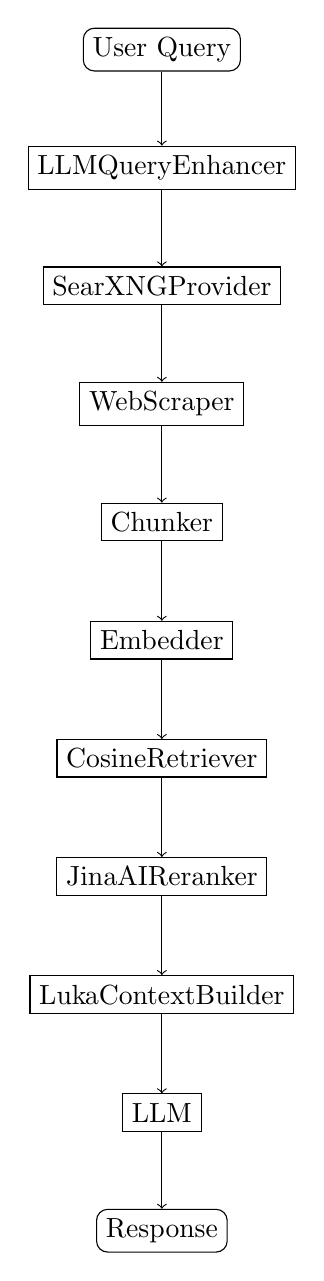
\begin{tikzpicture}[node distance=1.5cm]  
% Define the nodes  
\node (user) [draw, rounded corners] {User Query};  
\node (enhancer) [draw, below of=user] {LLMQueryEnhancer};  
\node (search) [draw, below of=enhancer] {SearXNGProvider};  
\node (scraper) [draw, below of=search] {WebScraper};  
\node (chunker) [draw, below of=scraper] {Chunker};  
\node (embedder) [draw, below of=chunker] {Embedder};  
\node (retriever) [draw, below of=embedder] {CosineRetriever};  
\node (reranker) [draw, below of=retriever] {JinaAIReranker};  
\node (context) [draw, below of=reranker] {LukaContextBuilder};  
\node (llm) [draw, below of=context] {LLM};  
\node (response) [draw, rounded corners, below of=llm] {Response};  
  
% Connect the nodes  
\draw[->] (user) -- (enhancer);  
\draw[->] (enhancer) -- (search);  
\draw[->] (search) -- (scraper);  
\draw[->] (scraper) -- (chunker);  
\draw[->] (chunker) -- (embedder);  
\draw[->] (embedder) -- (retriever);  
\draw[->] (retriever) -- (reranker);  
\draw[->] (reranker) -- (context);  
\draw[->] (context) -- (llm);  
\draw[->] (llm) -- (response);  
\end{tikzpicture}  
\caption{RAG Pipeline Architecture}  
\end{figure}  
  
\subsection*{Core Components}  
Our implementation consists of the following key components:  
  
\subsubsection*{Query Enhancement}
The search process transforms natural language queries into a set of optimized search expressions that search engines can process more effectively. The LLMQueryEnhancer component, powered by the self hosted LLama Nemotron-3 70B Large Language Model, performs this transformation by generating a configurable number of search queries (typically 3-5) that capture different aspects of the user's information need. For example, a user query "What are the latest developments in quantum computing?" might be transformed into structured search expressions like "quantum computing breakthroughs 2025", "recent quantum computer advancements site:.edu", and "quantum computing research papers after:2023".

The enhancement process employs several key strategies to maximize search effectiveness. The system considers temporal aspects, automatically incorporating time-based specifications when relevant. For technical queries, it preserves domain-specific terminology while adding relevant synonyms and related concepts. The enhancer also strategically employs advanced search operators, such as "site:", "after:", and exact phrase matching with quotation marks, to leverage the search engine's capabilities fully.

The system generates these enhanced queries through structured output generation, where the model produces a well-defined JSON format containing the optimized queries. This structured approach ensures consistent query formatting and enables systematic processing of different query aspects. The language-aware processing preserves the original query's language characteristics, including special characters and accents, while generating search expressions that align with search engine syntax.
  
\subsubsection*{Web Search and Content Acquisition}
The implementation utilizes a self-hosted SearXNG instance for web search functionality, operating as a meta search engine that aggregates results from multiple search providers. The SearXNGProvider component processes the enhanced queries generated in the previous stage and manages result acquisition through a REST API interface. The search parameters are configurable through a standardized configuration structure, allowing for precise control over result limits, language settings, and search engine selection.

The provider implements a systematic approach to result processing. Upon receiving enhanced queries, it executes parallel searches across multiple engines including Google, Bing, and DuckDuckGo. The system enforces configurable result limits, typically between 8-20 results per query, to maintain processing efficiency while ensuring adequate coverage. Each search operation returns a structured dataset comprising organic results, temporal information, and semantic relationships between queries.

Result normalization is performed through a defined transformation pipeline that converts heterogeneous source formats into a unified data structure. This structure preserves essential elements including titles, URLs, content snippets, and publication dates when available. The normalized format facilitates consistent downstream processing and enables systematic content extraction. Additional metadata, including related search terms and query suggestions, is preserved for potential query refinement and search space exploration.
  
\subsubsection*{Web Scraping Engine}
The WebScraper component processes the URLs obtained from the search phase through parallel execution, maximizing throughput while managing system resources. For each URL batch, the scraper initiates concurrent content extraction processes, implementing appropriate rate limiting and error handling to ensure reliable operation. The extracted HTML content undergoes a series of transformations, beginning with the removal of non-content elements through regular expression patterns targeting script tags, style definitions, and navigation components.

Following initial cleaning, the DefaultMarkdownGenerator processes the simplified HTML through DOM traversal, converting the hierarchical structure into standardized markdown format. This conversion preserves the semantic structure of headers, paragraphs, and lists while eliminating extraneous formatting. The PruningContentFilter examines each text segment against predefined patterns, systematically removing common web elements such as cookie notices and advertisements that do not contribute to the main content.

The resulting markdown undergoes further refinement through the MarkdownChunking algorithm, which segments content based on structural patterns in the text. This algorithm employs regular expressions to identify natural break points at markdown headers, horizontal rules, and paragraph breaks. To maintain content coherence, the algorithm enforces a minimum chunk size of 100 characters, automatically combining smaller segments with their neighbors. For Wikipedia sources, the system optimizes this process by bypassing HTML processing entirely, instead utilizing the Wikipedia API to obtain clean article text that is then converted directly to the standardized markdown format.

\subsubsection*{Content Processing Pipeline}
Building upon the initial markdown transformation, the content processing pipeline implements a series of refinement stages to optimize the text for retrieval. The process begins with the MarkdownChunking component, which analyzes the document structure using regular expressions. This component identifies and segments content at key structural points, maintaining chunk integrity by ensuring a minimum size threshold of 100 characters and intelligently merging undersized segments with adjacent content.

Content quality assessment follows through the QualityImprover component, which evaluates text at the paragraph level. The component preserves structural elements like code blocks (denoted by ```) while applying NVIDIA's DeBERTa-based quality classifier model. This model calculates quality scores on a three-point scale (Low=0, Medium=1, High=2), evaluating the educational value and information density of each content unit. The model considers various factors including word count (minimum 12 words per line), presence of substantive content, and filters out common UI elements and trading-related content. Content segments falling below the configurable quality threshold are filtered out, ensuring only high-value content progresses through the pipeline.

For example, UI elements like "SEARCH", "BOOK NOW", "GET A FREE QUOTE" are classified as low quality and filtered out, while informative news content with proper context and details is preserved as high quality.

The DefaultMarkdownGenerator then applies a systematic rule-based conversion, transforming the cleaned HTML into markdown while preserving the document's structural hierarchy and semantic relationships. Once the content is converted to clean markdown, it undergoes chunking to create manageable segments for retrieval.

\subsubsection*{Retrieval-Augmented Generation}
The cleaned markdown content is processed through our multi-stage retrieval system to identify the most relevant chunks for the user's query. First, the content is split into chunks of approximately 1000 characters with 100-character overlap to maintain context across boundaries. These chunks then flow through our retrieval pipeline:

\begin{enumerate}[noitemsep]
    \item \textbf{Initial Embedding}: Each chunk and the query are embedded using self-hosted BAAI's BGE-M2 (bge-multilingual-gemma2) model, chosen for its strong multilingual semantic understanding capabilities.
    
    \item \textbf{First-stage Retrieval}: The CosineRetriever performs an efficient initial filtering by computing cosine similarity between the query and chunk embeddings, selecting the top 50 most semantically similar chunks.
    
    \item \textbf{Cross-encoder Reranking}: These candidates undergo a more precise relevance assessment using the local JinaAI reranking model. This cross-encoder evaluates query-chunk pairs directly, providing more accurate relevance scores than pure embedding similarity.
    
    \item \textbf{Context Building}: The top 10 most relevant chunks after reranking are passed to the LukaContextBuilder, which assembles them into a coherent context for the llm while preserving source attribution and metadata.
\end{enumerate}

\subsubsection*{Context Building and Response Generation}
The context building phase transforms the processed markdown chunks into a structured format suitable for LLM consumption. The LukaContextBuilder manages this process by maintaining comprehensive metadata for each chunk, including source URLs, positional information, and quality scores. Each source is encapsulated in XML-style tags that include metadata:

\begin{verbatim}
<source url="..." id="1" relevance="0.39">
[Content of the chunk]
</source>
\end{verbatim}

To accommodate LLM token limitations, typically 4096 tokens, the builder implements dynamic context length management, ordering chunks by quality scores and applying necessary truncation while preserving content integrity. The final context is then passed to our self-hosted Nemotron-3 70B model with specific instructions to:
\begin{itemize}[noitemsep]
    \item Always cite sources using the provided URLs when making claims
    \item Maintain factual accuracy by strictly using information from the provided context
    \item Generate coherent responses that synthesize information across multiple sources
    \item Acknowledge when information is not available in the context
    \item Preserve source attribution in responses using markdown-style links
\end{itemize}

This structured approach ensures responses are both informative and traceable to their original sources while maintaining optimal context utilization within model limitations.

\subsection*{Conversation Management}
Our system maintains conversation history to support contextual follow-up queries. For follow-up questions, the system reuses previously embedded chunks from all the search results, performs retrieval and reranking on them based on the new query, builds new context from reranked chunks, and generates responses that consider previous conversation context. This approach enables natural, multi-turn conversations while maintaining factual accuracy.

\section*{Technical Implementation Details}
The implementation leverages the following models:

\begin{enumerate}[noitemsep]
    \item \textbf{Query Enhancement Model}\\
    Model: nvidia/Llama-3.1-Nemotron-70B-Instruct-HF\\
    Task: Generates multiple optimized search queries from user input
    
    \item \textbf{Content Quality Model}\\
    Model: nvidia/quality-classifier-deberta\\
    Task: Filters and scores content quality
    
    \item \textbf{Embedding Model}\\
    Model: BAAI/bge-multilingual-gemma2\\
    Task: Generates semantic embeddings for chunks and queries
    
    \item \textbf{Reranking Model}\\
    Model: jina-ai/reranker-v2\\
    Task: Cross-encoder reranking of retrieved chunks
    
    \item \textbf{Language Model}\\
    Model: nvidia/Llama-3.1-Nemotron-70B\\
    Task: Response generation and synthesis
\end{enumerate}

All models are self-hosted or run locally, using VLLM inference server for the LLM and huggingface transformers for reranking and content quality classification.

\subsection*{Evaluation Methodology}
To evaluate our RAG system's performance, we conducted extensive testing using the SimpleQA dataset, comprising 1000 carefully curated question-answer pairs. The evaluation focused on assessing both the system's ability to retrieve relevant information and generate accurate responses across different types of questions.

\subsubsection*{Experimental Setup}
Our experiments were conducted using the following system parameters:
\begin{itemize}[noitemsep]
    \item \textbf{Query Enhancement}: Maximum of 3 enhanced queries per user question
    \item \textbf{Web Search}: Maximum of 10 sources retrieved per query
    \item \textbf{Content Processing}: 1000-character chunks with 100-character overlap
    \item \textbf{Retrieval}: Top-50 initial candidates, refined to top-20 after reranking
    \item \textbf{Models}: BAAI/bge-multilingual-gemma2 for embeddings, Nemotron-3 70B for LLM
    \item \textbf{Quality Filter}: Content quality classifier with configurable threshold (enabled/disabled)
\end{itemize}

\subsubsection*{Experimental Design}
We conducted three distinct experiments to evaluate different system configurations:

\begin{enumerate}[noitemsep]
    \item \textbf{Plain LLM}: Baseline using only the large language model without any retrieval augmentation
    \item \textbf{Ours}: Our complete RAG search pipeline with real-time web scraping and content processing
    \item \textbf{Ours + Quality Filter}: Our system enhanced with content quality filtering to remove low-quality web content
\end{enumerate}

\subsubsection*{Dataset and Evaluation Process}
The SimpleQA dataset includes a diverse range of questions covering various topics and answer types, including:
\begin{itemize}[noitemsep]
    \item Person identification (e.g., "Who is the CEO of...?")
    \item Date-based queries (e.g., "When was...?")
    \item Numerical answers (e.g., "How many...?")
    \item Location information (e.g., "Where is...?")
    \item Other factual information
\end{itemize}

\subsubsection*{Grading Methodology}
We employed a rigorous automated grading system using a large language model to evaluate response accuracy. The grading system categorized each response into one of three categories:

\begin{itemize}[noitemsep]
    \item \textbf{Correct (A)}: Responses that fully contain the important information from the gold target without contradictions. This includes answers that may have additional context but maintain factual accuracy.
    \item \textbf{Incorrect (B)}: Responses containing any factual contradictions with the gold target, even if presented with hedging language.
    \item \textbf{Not Attempted (C)}: Responses that neither confirm nor contradict the gold target, including explicit acknowledgments of uncertainty.
\end{itemize}

The grading system was particularly nuanced in handling:
\begin{itemize}[noitemsep]
    \item Numerical answers (accepting ±1\% margin of error)
    \item Partial information when complete context can be inferred from the question
    \item Name variations and minor typographical errors
    \item Context-dependent completeness of answers
\end{itemize}

\textbf{Evaluation Limitation:} It should be noted that we used the same LLM family (Nemotron-3 70B) for both response generation and evaluation. While this ensures consistency in evaluation criteria, human-checked results could potentially differ by a few percentage points due to different interpretation standards and subjective judgment in edge cases.

\subsection*{Results and Analysis}

Our experimental evaluation demonstrates the significant impact of retrieval-augmented generation on question-answering performance. Figure \ref{fig:accuracy_comparison} presents the overall accuracy comparison across our three experimental configurations, while Figure \ref{fig:grade_distribution} shows the detailed distribution of response quality categories.

\begin{figure}[h]
\centering
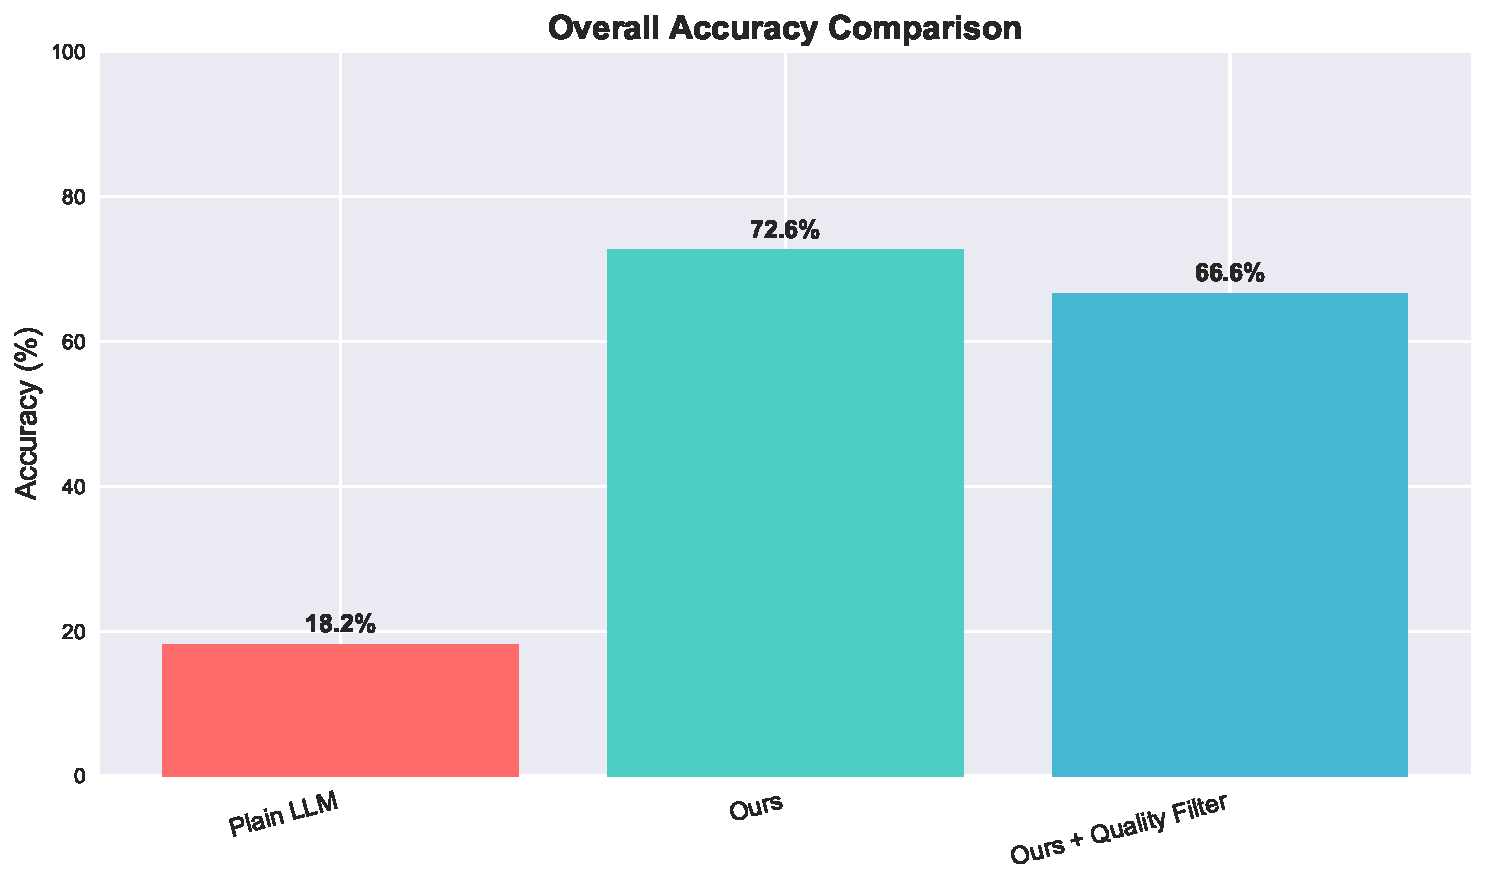
\includegraphics[width=0.5\textwidth]{accuracy_comparison.pdf}
\caption{Overall accuracy comparison across experimental configurations. Our RAG search pipeline achieves 72.6\% accuracy compared to 18.2\% for the plain LLM baseline, representing significantimprovement.}
\label{fig:accuracy_comparison}
\end{figure}

\begin{figure}[h]
\centering
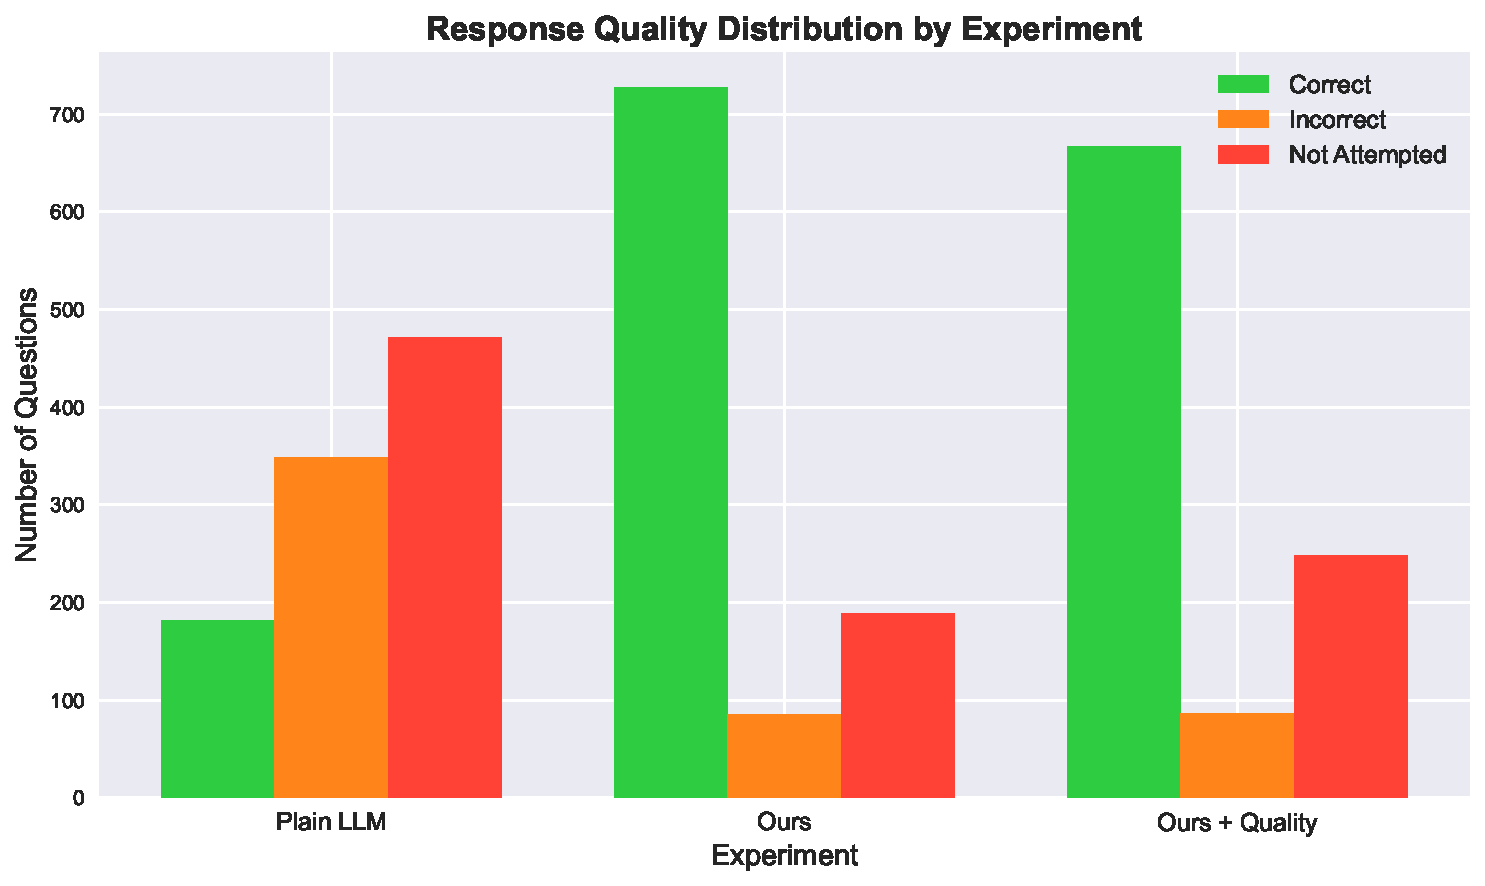
\includegraphics[width=0.5\textwidth]{grade_distribution.pdf}
\caption{Distribution of response quality across experiments. The chart shows the number of questions receiving Correct (A), Incorrect (B), or Not Attempted (C) grades for each system configuration.}
\label{fig:grade_distribution}
\end{figure}

\subsubsection*{Performance Results}
The experimental results reveal substantial performance improvements when incorporating real-time web retrieval:

\begin{itemize}[noitemsep]
    \item \textbf{Plain LLM}: Achieved only \textbf{18.2\% accuracy} (182/1001 questions correct), with 47.1\% of questions not attempted and 34.8\% answered incorrectly
    \item \textbf{Ours}: Reached \textbf{72.6\% accuracy} (727/1001 questions correct), representing a substantial improvement over the baseline
    \item \textbf{Ours + Quality Filter}: Obtained \textbf{66.6\% accuracy} (667/1001 questions correct), showing decreased performance compared to the unfiltered system
\end{itemize}

\subsubsection*{Impact Analysis}
Our experiments clearly demonstrate that our RAG search pipeline significantly enhances LLM performance on factual question answering. The plain LLM achieved 18.2\% accuracy, while our complete pipeline achieved 72.6\% accuracy, showing that our system performs substantially better. This validates the effectiveness of real-time web retrieval and content processing in providing LLMs with current, relevant information.

Interestingly, we discovered that filtering paragraphs and links from scraped web content actually degraded performance. The quality-enhanced version achieved 66.6\% accuracy compared to 72.6\% without filtering, indicating that the unfiltered system performed better. This suggests that the content quality classifier may have been overly conservative, removing potentially useful information alongside low-quality content.

\subsubsection*{Custom Dataset Evaluation}
To further validate our system's capabilities, we created a separate curated dataset of 100 questions that we came up with ourselves, covering diverse topics and query types. Our pipeline performed exceptionally well on this custom dataset, achieving \textbf{92\% accuracy} (92 out of 100 questions correct). This high performance on hand-curated questions demonstrates the system's robustness across different question types and domains.

Notably, the system performed effectively even on Slovenian queries, showcasing its multilingual capabilities and the effectiveness of our multilingual embedding model (BAAI/bge-multilingual-gemma2) in handling non-English content retrieval and processing.

\subsubsection*{System Reliability}
Our analysis identified consistent performance patterns across different question types. The substantial improvement from 18.2\% to 72.6\% accuracy validates our core hypothesis that real-time web retrieval significantly enhances LLM performance on knowledge-intensive tasks. The system's ability to achieve over 92\% accuracy on curated samples while maintaining strong performance on large-scale evaluation demonstrates its practical value for real-world applications.

\section*{Conclusion}

This work presents a comprehensive implementation of a conversational agent enhanced with real-time Retrieval-Augmented Generation capabilities. Our system successfully addresses the fundamental limitations of traditional LLMs by incorporating dynamic web scraping and intelligent content processing to provide accurate, up-to-date responses to factual questions.

\subsubsection*{Key Contributions}
Our research makes several significant contributions to the field of conversational AI:

\begin{enumerate}[noitemsep]
    \item \textbf{Real-time RAG Architecture}: We developed a modular, end-to-end pipeline that seamlessly integrates query enhancement, web search, content extraction, and response generation, all using self-hosted open-source components.
    
    \item \textbf{Performance Validation}: Our experiments demonstrate the critical value of external knowledge retrieval for factual question answering, with substantial improvements over baseline LLM performance.
    
    \item \textbf{Multilingual Capabilities}: The system effectively handles queries in multiple languages, including Slovenian, showcasing its versatility for diverse linguistic contexts.
    
    \item \textbf{Quality vs. Coverage Insights}: We identified that aggressive content filtering can degrade performance, providing valuable guidance for future RAG system design.
\end{enumerate}

\subsubsection*{Practical Implications}
The substantial performance improvements validate the practical value of real-time web retrieval for knowledge-intensive applications. Our system's strong performance on both large-scale benchmarks and curated questions demonstrates its readiness for real-world deployment. The fully self-hosted architecture ensures data privacy and control, making it suitable for enterprise applications.

\subsubsection*{Limitations and Future Work}
While our results are promising, several limitations warrant consideration. The evaluation relied on automated LLM-based grading, which may differ from human judgment. Additionally, the system's performance depends on web content quality and availability, and processing latency may impact real-time user experience.

Future research directions include optimizing quality filtering mechanisms, exploring more sophisticated query enhancement strategies, and investigating the integration of structured knowledge bases alongside web scraping to further improve accuracy and response completeness.

Our work demonstrates that real-time RAG systems can significantly enhance conversational AI capabilities, providing a practical foundation for next-generation knowledge-augmented chatbots and virtual assistants.

\textbf{Additional Contribution:} During our project development, we identified and contributed to fixing a critical bug in SearXNG, the open-source meta-search engine used in our pipeline. Our detailed bug report and proposed fix for the currency processor issue was accepted and merged into the main project \cite{searxng_bug}.

\bibliographystyle{unsrt}
\bibliography{report}

\end{document}